% !TEX TS-program = pdflatexmk
\documentclass[12pt]{article}

% Layout.
\usepackage[top=1in, bottom=0.75in, left=1in, right=1in, headheight=1in, headsep=6pt]{geometry}

% Fonts.
\usepackage{mathptmx}
\usepackage[scaled=0.86]{helvet}
\renewcommand{\emph}[1]{\textsf{\textbf{#1}}}

% TiKZ.
\usepackage{tikz, pgfplots}
\usetikzlibrary{calc}
\pgfplotsset{my style/.append style={axis x line=middle, axis y line=
middle, xlabel={$x$}, ylabel={$y$}, axis equal }}

% Misc packages.
\usepackage{amsmath,amssymb,latexsym}
\usepackage{graphicx}
\usepackage{array}
\usepackage{xcolor}
\usepackage{multicol}

% Commands to set various header/footer components.
\makeatletter
\def\doctitle#1{\gdef\@doctitle{#1}}
\doctitle{Use {\tt\textbackslash doctitle\{MY LABEL\}}.}
\def\docdate#1{\gdef\@docdate{#1}}
\docdate{Use {\tt\textbackslash docdate\{MY DATE\}}.}
\def\doccourse#1{\gdef\@doccourse{#1}}
\let\@doccourse\@empty
\def\docscoring#1{\gdef\@docscoring{#1}}
\let\@docscoring\@empty
\def\docversion#1{\gdef\@docversion{#1}}
\let\@docversion\@empty
\makeatother

% Headers and footers layout.
\makeatletter
\usepackage{fancyhdr}
\pagestyle{fancy}
\fancyhf{} % Clears all headers/footers.
\lhead{\baselineskip 30pt
\emph{\@doctitle\hfill\@docdate}
\ifnum \value{page} > 1\relax\else\\
\emph{Name: \rule{3.5in}{1pt}\hfill \@docscoring}\fi}
\rfoot{\emph{\@docversion}}
\lfoot{\emph{\@doccourse}}
\cfoot{\emph{\thepage}}
\renewcommand{\headrulewidth}{0pt}%
\makeatother

% Paragraph spacing
\parindent 0pt
\parskip 6pt plus 1pt

% A problem is a section-like command. Use \problem{5} to
% start a problem worth 5 points.
\newcounter{probcount}
\newcounter{subprobcount}
\setcounter{probcount}{0}
\newcommand{\problem}[1]{%
\par
\addvspace{4pt}%
\setcounter{subprobcount}{0}%
\stepcounter{probcount}%
\makebox[0pt][r]{\emph{\arabic{probcount}.}\hskip1ex}\emph{[#1 points]}\hskip1ex}
\newcommand{\thesubproblem}{\emph{\alph{subprobcount}.}}

% Subproblems are an enumerate-like environment with a consistent
% numbering scheme. 
% Use \begin{subproblems}\item...\item...\end{subproblems}
\newenvironment{subproblems}{%
\begin{enumerate}%
\setcounter{enumi}{\value{subprobcount}}%
\renewcommand{\theenumi}{\emph{\alph{enumi}}}}%
{\setcounter{subprobcount}{\value{enumi}}\end{enumerate}}

% Blanks for answers in normal and math mode.
\newcommand{\blank}[1]{\rule{#1}{0.75pt}}
\newcommand{\mblank}[1]{\underline{\hspace{#1}}}
\def\emptybox(#1,#2){\framebox{\parbox[c][#2]{#1}{\rule{0pt}{0pt}}}}

% Misc.
\renewcommand{\d}{\displaystyle}
\newcommand{\ds}{\displaystyle}
\def\bc{\begin{center}}
\def\ec{\end{center}}
\def\be{\begin{enumerate}}
\def\ee{\end{enumerate}}


\doctitle{Math 251: Quiz 2}
\docdate{September 10, 2019}
\doccourse{UAF Calculus I}
\docversion{v-1}
\docscoring{\blank{0.8in} / 25}
\begin{document}
\textbf{Please circle your instructor's name:} \hfill Leah Berman  \hfill   Jill Faudree\\

There are 25 points possible on this quiz. No aids (book, calculator, etc.)
are permitted.  Show all work for full credit.

\problem{9}
Use the graph of the function of $f(x)$ to answer the following questions.\\
\begin{center}
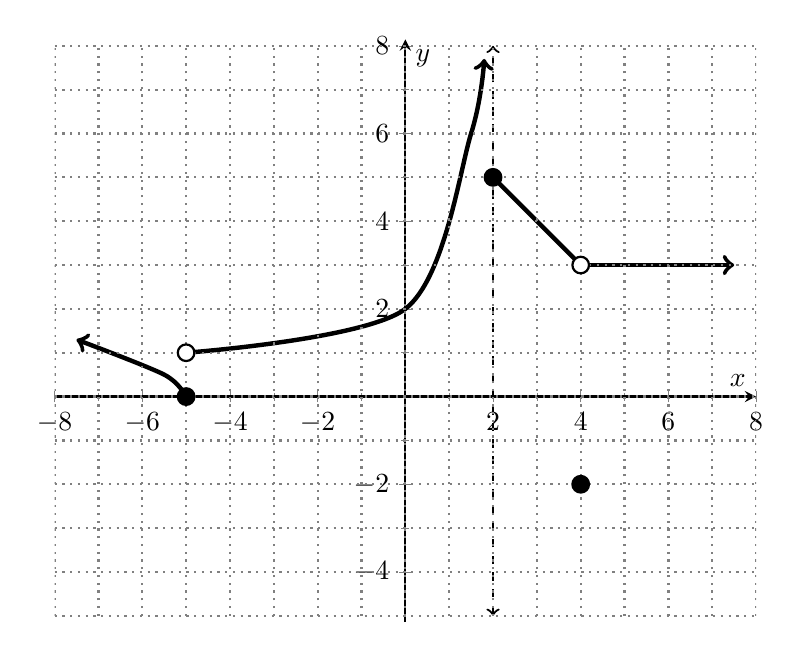
\begin{tikzpicture}
\begin{axis}[scale=1.3, thick, my style, xtick={-8,-6,...,8}, ytick={-4,-2,...,8},
xmin=-8, xmax=8, ymin=-5, ymax=8, minor y tick num=1,
        minor x tick num=1, mark size=3.0pt]
%asymptote
\addplot[dashed,<->, thick] coordinates {(2,-5) (2,8)};
%points solid
\addplot[mark=*,only marks] coordinates {(-5,0)(2,5)(4,-2)};
%points open
\addplot[mark=*,fill=white,only marks] coordinates {(-5,1)
(4,3)};
\addplot[ultra thick, smooth,->] coordinates {(-5,0) (-5.5,.5)(-7.5,1.3)};
\addplot[ultra thick, smooth] coordinates {(2,5) (4,3)};
\addplot[ultra thick, smooth,->] coordinates {(4,3) (7.5,3)};
\addplot[ultra thick, smooth,->] coordinates {(-5,1) (0,2) (1.5,6) (1.8,7.7)};
%\addplot[domain=5:8,->,ultra thick] {1};
%\addplot[domain=0:5, -, ultra thick] {3 - 2*x/5 };
%\addplot[domain=-3.98:0,<-, ultra thick] {max(2-2/sqrt(((4+x))),-4)};
%% \addplot[domain=3:4.87,->, ultra thick]{3.5+(x-5)^(-1)};
%\addplot[domain=-8:-4.01,<->, ultra thick]{min((6+x)/sqrt(-x-4),8)};
%\addplot[mark=*,only marks] coordinates {(5,4)(0,1)};
%\addplot[mark=*,fill=white,only marks] coordinates {(5,1)
%(0,3)};
\foreach \i in {-8,-7,-6,...,8}{
	\addplot[dotted, gray, domain=-8:8]{\i};
	\addplot[dotted, gray] coordinates {(\i,-5) (\i,8)};
	}
\end{axis}
\end{tikzpicture}
\end{center}

\begin{subproblems}
\begin{multicols}{3}
\item $\d{\lim_{x \to -5^-} f(x)=\mblank{.5in}}$
\item $\d{\lim_{x \to -5^+} f(x)=\mblank{.5in}}$
\item $\d{\lim_{x \to -5} f(x)=\mblank{.5in}}$
\end{multicols}
\begin{multicols}{3}
\item $f(-5)=\mblank{.5in}$
\item $f(2)=\mblank{.5in}$
\item $f(4)=\mblank{.5in}$
\end{multicols}
\begin{multicols}{3}
\item $\d{\lim_{x \to 0} f(x)=\mblank{.5in}}$
\item $\d \lim_{x\to 2^-}f(x)=\mblank{.5in}$
\item $\d{\lim_{x \to 4} f(x)=\mblank{.5in}}$
\end{multicols}
\end{subproblems}


\problem{4} An empty tank can hold 2000 gallons of water  and is filled in one hour. The values in the table show the volume $V$ of water  in the tank (in gallons) after $t$ minutes.
\begin{center}
\begin{tabular}{|c|c|c|c|c|c|c|c|}
\hline
$t$ (minutes) &0&10&20&30&40&50&60 \\
\hline
$V$ (gallons) &0& 200& 500&1100 & 1500&1800&2000 \\
\hline
\end{tabular}
\end{center}

\begin{subproblems}
\item Find the average rate of change of the water in the tank in the first half of an hour. Include units in your answer.
\vskip 2cm

\item During what 10 minute interval was the average rate of change of the water the greatest (in magnitude)?
\end{subproblems}
\vskip 2cm



\newpage
\problem{6} Compute the following infinite limits. For each limit, justify your answer 
with a sentence or two, perhaps with a rough sketch.
\begin{subproblems}
\item$\d \lim_{x\rightarrow 8^+} -2 \ln (x-8)=\emptybox(40pt,30pt)$
\vskip 3cm

\item$\d \lim_{x\rightarrow \pi^+} \frac{x+1}{\pi - x}=\emptybox(40pt,30pt)$
\vskip 3cm
\end{subproblems}


\problem{6} On the axes below, sketch the graph of the function 
\[
f(x)=\begin{cases} 
4+x & x < 0\\
3 & x = 0\\
e^x & x > 0.
\end{cases}
\]

Then compute, with brief justification, the requested values in the table.

\begin{multicols}{2}

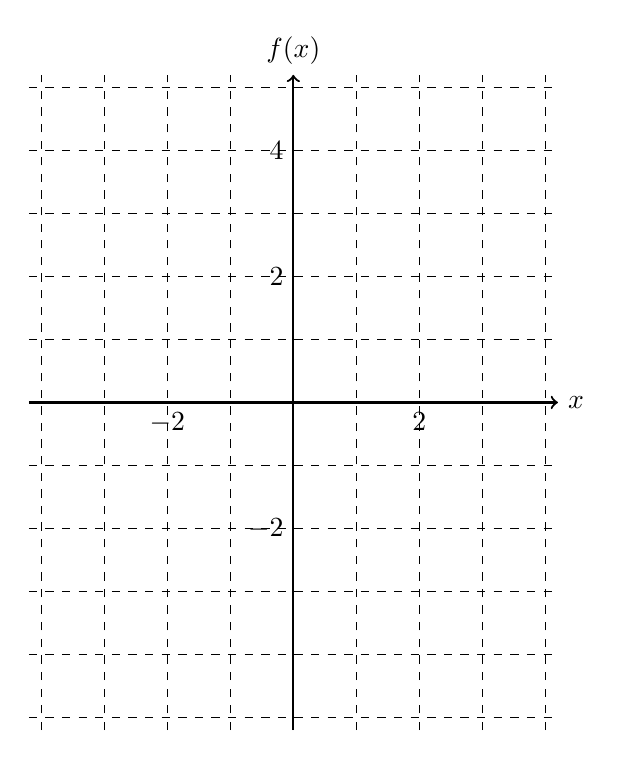
\begin{tikzpicture}[scale=0.8]
\draw [%help lines,
dashed] (-4.2,-5.2) grid (4.2,5.2);
\draw [thick, ->] (-4.2,0)--(4.2,0) node[right] {$x$};
\draw [thick, ->] (0,-5.2)--(0,5.2) node[above]{$f(x)$};
\foreach \i in {-2,2}
{	\node[below] at (\i,0) {$\i$};
}
\foreach \i in {-2,2,4}
{	\node[left] at (0,\i) {$\i$};
}
\end{tikzpicture}

\columnbreak

\begin{tabular}{|c|c|}\hline
Value & Justification \\ \hline
$f(0)=$ &\raisebox{10pt}{\parbox[t][0.8in]{2.5in}{\strut}}\\ \hline
$\d \lim_{x\rightarrow 0^-} f(x)=$  &\raisebox{20pt}{\parbox[t][1.2in]{2.5in}{}}\\\hline
$\d \lim_{x\rightarrow 0} f(x)=$    &\raisebox{20pt}{\parbox[t][1.2in]{2.5in}{}} \\ \hline
\end{tabular}
\end{multicols}

\end{document}